\section{Background}
\label{sec:background}

\subsection{Parallel and Perpendicular Decomposition}
\label{sec:decomp}

Let $\mathbf{z}, \Delta \in \mathbb{R}^d$ with $\mathbf{z} \neq \mathbf{0}$.
The update $\Delta$ decomposes uniquely into a component parallel to
$\mathbf{z}$ and a component perpendicular to it:
\begin{align}
  \Delta_\parallel
    &= \frac{\Delta \cdot \mathbf{z}}{\|\mathbf{z}\|^2}\,\mathbf{z}
     = \alpha\,\mathbf{z},
     \qquad
     \alpha = \frac{\Delta \cdot \mathbf{z}}{\|\mathbf{z}\|^2},
  \label{eq:para} \\
  \Delta_\perp
    &= \Delta - \Delta_\parallel,
    \qquad \Delta_\perp \perp \mathbf{z}.
  \label{eq:perp}
\end{align}
The parallel component $\Delta_\parallel$ rescales $\mathbf{z}$ without
changing its direction. The perpendicular component $\Delta_\perp$ lives in
the $(d-1)$-dimensional subspace orthogonal to $\mathbf{z}$ and carries the
direction-changing degrees of freedom.

This decomposition is the sole mathematical tool used throughout the paper.
In \S\ref{sec:method} we apply it at two levels within a transformer:
to the block's residual output in the hidden-state space (\S\ref{sec:residual-level}),
and to the value projection in the attention's internal representation space
(\S\ref{sec:value-level}).

\subsection{Transformer Residual Updates}
\label{sec:transformer}

We consider transformer residual streams with $L$ layers and hidden dimension
$d$. Each residual sub-layer adds an update to the current representation:
\begin{equation}
  \hl{l+1} = \hl{l} + \Dl{l},
  \label{eq:residual}
\end{equation}
The update $\Dl{l}$ may denote the output of a multi-head self-attention
($\Attn$) sub-layer, a feed-forward ($\FFN$) sub-layer, or their combined
block-level contribution.
We write $\hz{l}{t}$ for the hidden state at layer $l$, token position
$t \in \{1,\ldots,T\}$, and $\Du{l}{t}$ for the corresponding residual update.

Using eq.~\ref{eq:para}, the parallel part of a residual update is
\begin{equation}
  \Dup{l}{t} = \alpha^l_t \hz{l}{t}, \qquad
  \alpha^l_t = \frac{\Du{l}{t}\cdot \hz{l}{t}}{\|\hz{l}{t}\|^2},
\end{equation}
so the parallel component is equivalent to a token-wise scaling of the
existing hidden state. The residual update can therefore be written as
\begin{equation}
  \hz{l+1}{t}
  = (1+\alpha^l_t)\hz{l}{t} + \Duperp{l}{t}, \qquad
  \Duperp{l}{t}\perp \hz{l}{t}.
\end{equation}

To measure update geometry in Figure~\ref{fig:profiles}, we report the
relative magnitude $\|\Dup{l}{t}\|/\|\Duperp{l}{t}\|$ across sampled layers.
This ratio compares the direction-preserving part of the update with its
direction-changing part.

\begin{figure}[t]
  \centering
  \begin{subfigure}{0.49\linewidth}
    \centering
    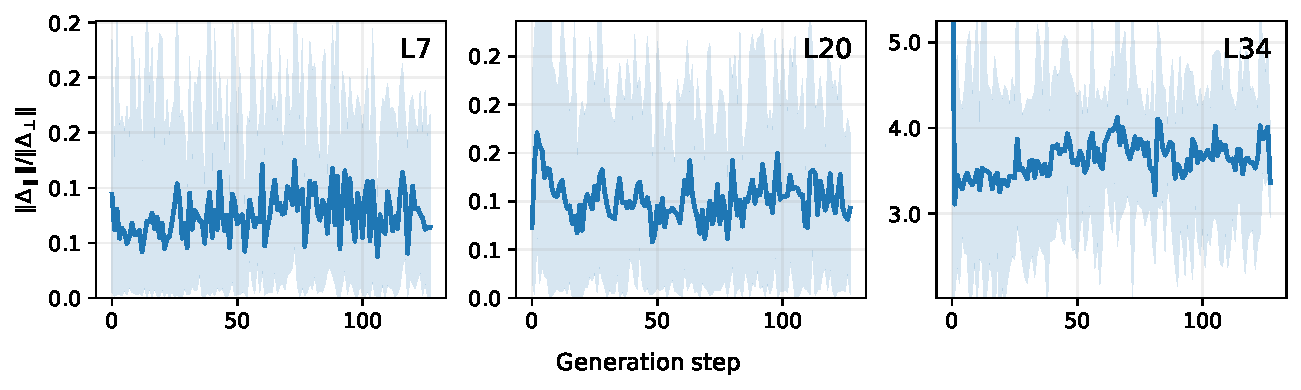
\includegraphics[width=\linewidth]{figs/para_dist/paper_Qwen3-4B_hidden_both_block_para_perp_sampled_layers.pdf}
    \caption{Qwen3-4B}
  \end{subfigure}
  \begin{subfigure}{0.49\linewidth}
    \centering
    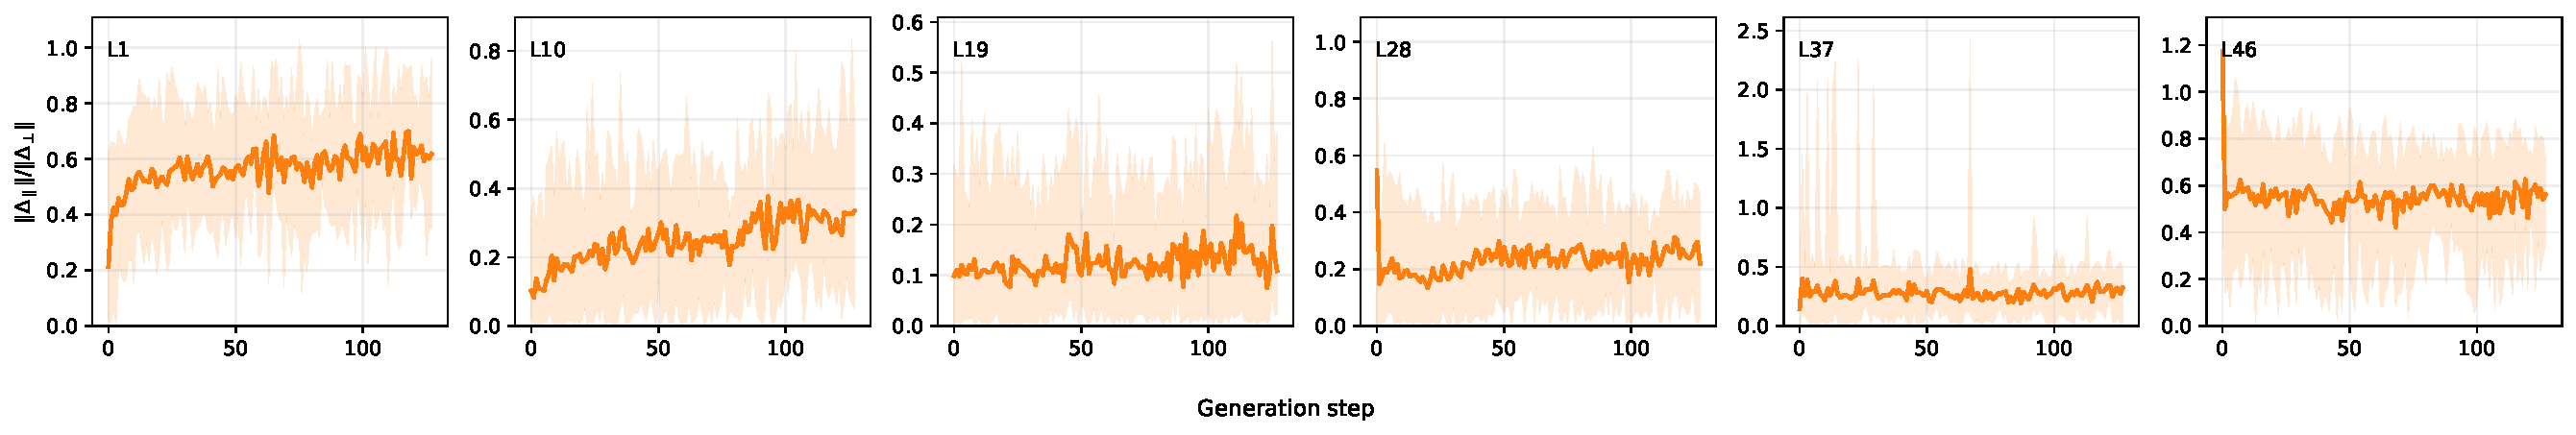
\includegraphics[width=\linewidth]{figs/para_dist/paper_Qwen3-30B-A3B_hidden_both_block_para_perp_sampled_layers.pdf}
    \caption{Qwen3-30B-A3B}
  \end{subfigure}
  \caption{\textbf{Parallel and perpendicular component ratios across depth.}
           Layerwise residual-update geometry at sampled layers for Qwen3-4B
           and Qwen3-30B-A3B, measured by the relative magnitude
           $\|\Dup{l}{t}\|/\|\Duperp{l}{t}\|$. In both models, the parallel
           component remains substantial relative to the perpendicular
           component across depth, motivating the later analysis of its
           functional role.}
  \label{fig:profiles}
\end{figure}

Figure~\ref{fig:profiles} establishes the empirical pattern used throughout
the paper: many residual updates have a substantial parallel component
relative to their perpendicular component across depth. Subsequent sections
analyze the source of this geometry and the effect of interventions that
modify it.
